\newpage
\section{Results and Analysis}\label{sec:result}

\subsection{Comparison of the Four Classifiers}
All four classifiers were trained on the same feature set and evaluated with LOSO cross-validation over the 3 group members. Table~\ref{tab:model_comparison} summarizes the overall mean accuracy and its standard deviation across the three folds.

\begin{table}[!htb]
    \centering
    \caption{LOSO cross-validation accuracy of the four classifiers}
    \label{tab:model_comparison}
    \begin{tabularx}{\textwidth}{@{} l l l X @{}}
        \toprule
        \textbf{Model} & \textbf{Mean Accuracy} & \textbf{Std.} & \textbf{Remarks} \\
        \midrule
        MLP & 0.795 & $\pm$ 0.099 & Per subject (B12901057 / 059 / 069): 0.676 / 0.919 / 0.790. \\
        SVM & 0.811 & $\pm$ 0.097 & Second best, with $C=0.01$; per subject: 0.729 / 0.948 / 0.757. \\
        RF  & 0.751 & $\pm$ 0.121 & Lowest of the four; per subject: 0.624 / 0.914 / 0.714. \\
        Shrinkage LDA (self-selected) & \textbf{0.825} & $\pm$ 0.101 & Best model; per subject: 0.705 / 0.952 / 0.819. \\
        \bottomrule
    \end{tabularx}
\end{table}

\noindent Shrinkage LDA performed best with a mean accuracy of 0.825, which is 1.4, 3.0 and 7.4 percentage points higher than the SVM, MLP and RF, respectively. The hyperparameters of the three given classifiers were selected by the parameter experiments of Section~\ref{sec:method}, so these numbers are the best settings found, not the framework's initial values; the MLP and the Random Forest average $0.793 \pm 0.009$ and $0.758 \pm 0.006$ over ten random seeds (Appendix~\ref{app:app02}), so their numbers vary by about one percentage point with the seed. All four classifiers reached the 75\% target, and the best two (LDA and SVM) also exceed 80\%. The standard deviation is the (population) standard deviation of the three fold accuracies, i.e.\ it reflects the difference between the three members rather than the randomness of a single run.

\subsection{Effect of Preprocessing and Feature Engineering}
To quantify how much of the performance comes from the processing pipeline rather than from the classifier itself, we compare a reference configuration against our final pipeline. The reference configuration feeds the raw 8~s time-domain samples (4096 values per segment) directly to the four classifiers, with no filtering and no normalization. We then add exactly one step at a time: band-pass filtering of the raw samples, the window-based band-power features, the time-domain features, and finally the subject-wise z-score, which stays off until the last step. All other settings (segmentation, hyperparameters, LOSO folds) are identical in every row. For every row the table reports the accuracy of the best of the four models, which is a different model in different rows (SVM, LDA, MLP, LDA), so the accuracy of every model is given in Appendix~\ref{app:app02}. The script \texttt{ablation.py} in the repository reproduces this table.

\begin{table}[!htb]
    \centering
    \caption{Ablation study of the processing pipeline (accuracy of the best model)}
    \label{tab:ablation}
    \begin{tabularx}{\textwidth}{@{} >{\raggedright\arraybackslash}p{0.33\textwidth} l X @{}}
        \toprule
        \textbf{Configuration} & \textbf{Mean Accuracy} & \textbf{Observation} \\
        \midrule
        Raw time-domain samples & 0.500 (SVM) & Reference; 4096-dimensional input, chance level is 0.333. \\
        + Band-pass filtering (1--45~Hz, 60~Hz notch) & 0.537 (SVM) & +3.7 points; the raw samples remain high-dimensional and phase-dependent. \\
        + Window band-power features & 0.571 (LDA) & +3.4 points; compact spectral features are far better than raw samples. \\
        + Time-domain features (std, kurtosis) & 0.700 (MLP) & +12.9 points; amplitude and spikiness separate Stroop from the others. \\
        + Subject-wise z-score (final pipeline) & \textbf{0.825} (LDA) & +12.5 points; as large as the time-domain features. \\
        \midrule
        \emph{Extra:} band power + z-score & 0.803 (LDA) & Not a cumulative step; shows that the z-score alone lifts the band-power features from 0.571 to 0.803, and the time-domain features add the last 2.2 points. \\
        \bottomrule
    \end{tabularx}
\end{table}

\subsection{Detailed Results of the Best Model}
Figure~\ref{fig:final_results} shows the results of our final run.

\noindent The terminal output summary of the same run (\texttt{results\_summary.txt}) is:
\begin{verbatim}
Summary of Classification Results (LOSO):
 - MLP         : 0.795 +/- 0.099
 - SVM         : 0.811 +/- 0.097
 - RF          : 0.751 +/- 0.121
 - SelfSelected: 0.825 +/- 0.101

Best Performing Model: SelfSelected with Accuracy 0.825
  -> reached the 75% target

Accuracy per held-out subject:
Subject                    MLP           SVM            RF  SelfSelected
b12901057                0.676         0.729         0.624         0.705
b12901059                0.919         0.948         0.914         0.952
b12901069                0.790         0.757         0.714         0.819

Detailed Class Report for Best Model [SelfSelected]:
[Relax Class]
  - Accuracy (Recall): 0.781 (164/210)
  - Precision: 0.820 (164/200)
  - F1-score: 0.800

[Focus Class]
  - Accuracy (Recall): 0.829 (174/210)
  - Precision: 0.777 (174/224)
  - F1-score: 0.802

[Stroop Class]
  - Accuracy (Recall): 0.867 (182/210)
  - Precision: 0.883 (182/206)
  - F1-score: 0.875

Overall Confusion Matrix [SelfSelected] (rows = true, cols = predicted):
               Relax     Focus    Stroop
Relax            164        34        12
Focus             24       174        12
Stroop            12        16       182
\end{verbatim}

\begin{figure}[H]
    \centering
    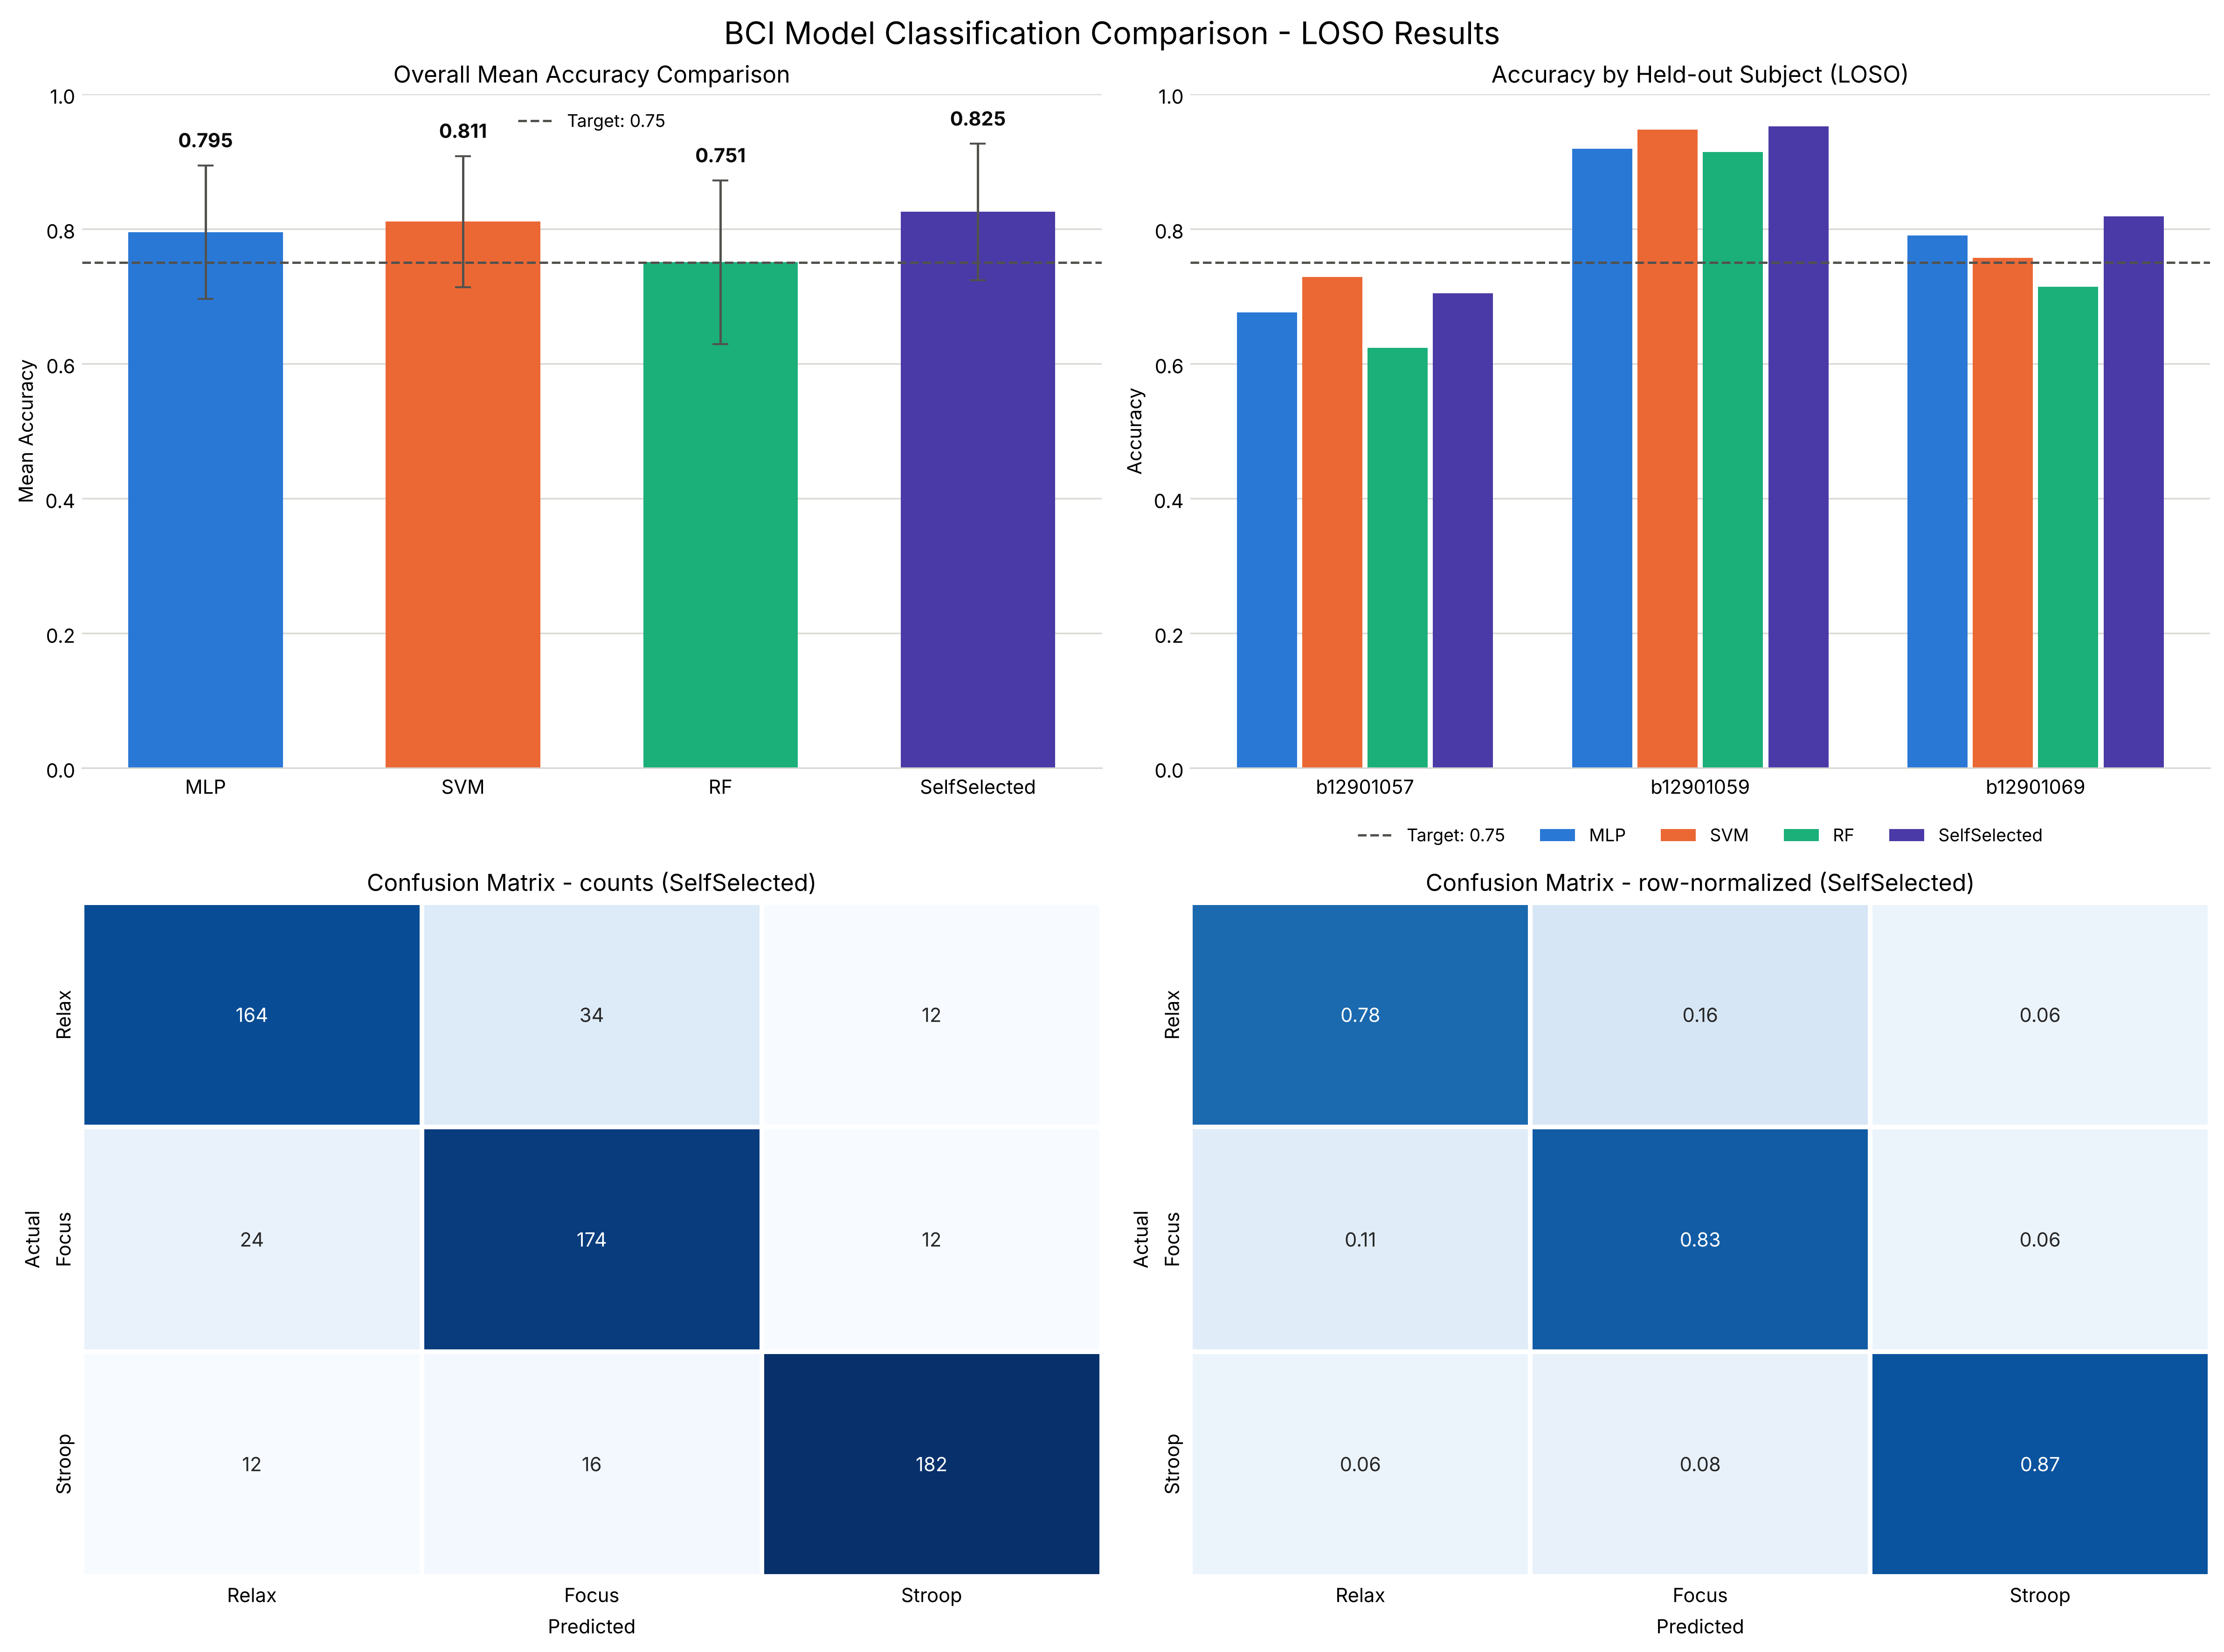
\includegraphics[width=\linewidth]{figures/bci_multi_model_comparison.png}
    \caption{LOSO cross-validation results of the best model, including the accuracy of the four models, the per-subject accuracy for the 3 group members, and the overall $3 \times 3$ confusion matrix.}
    \label{fig:final_results}
\end{figure}

\subsection{Result Analysis and Discussion}
\begin{itemize}[leftmargin=*]
    \item \textbf{Accuracy Comparison:} Shrinkage LDA (0.825) $>$ SVM (0.811) $>$ MLP (0.795) $>$ RF (0.751); all of them reached the $\geq 75\%$ target, and the best two models (LDA and SVM) also exceeded 80\%. LDA suits this dataset for three reasons. After the subject-wise z-score, the class differences are mostly shifts of the mean of a few band features (Relax has the highest relative alpha, Focus the highest relative beta, Stroop the highest amplitude and theta; class means of the z-scored features over all three members, see below), which a linear boundary can separate. There are only 420 training samples for 32 features, so a model with few parameters and automatic covariance shrinkage is less prone to over-fitting than the MLP or the RF. Finally, LDA has no hyperparameter that needs tuning on only three folds.
    \item \textbf{Confusion Matrix Analysis:} Using the $3 \times 3$ confusion matrix in Figure~\ref{fig:final_results}:
    \begin{itemize}
        \item \emph{Easiest class: Stroop} (recall 0.867, precision 0.883). Its z-scored amplitude and kurtosis are the highest (+0.89 and +0.98 versus $-0.55$/$-0.59$ for Relax), and its relative theta and $\theta/\beta$ are also the highest. Stroop has the highest amplitude in each of the three members (z-scored log standard deviation $+0.67$ to $+1.06$), not only on average. This fits the expectation that reading the words and answering with the keyboard add eye and muscle activity at Fp1, on top of the frontal theta that accompanies cognitive conflict~\cite{cavanagh2014}. With one channel, however, we cannot tell how much of the amplitude is cortical and how much is artifact.
        \item \emph{Most confused pair: Relax and Focus.} 34 Relax segments were predicted as Focus and 24 Focus segments as Relax (58 errors), compared with 28 errors between Focus and Stroop and 24 between Relax and Stroop. Both states have a below-average amplitude (z-scored log standard deviation $-0.55$ and $-0.34$), and they differ mainly in the balance between alpha (higher in Relax, +0.95) and beta (higher in Focus), which is subtle at a single frontal electrode.
        \item \emph{Effect of our processing.} Counting the Relax and Focus errors of LDA at each ablation step (Table~\ref{tab:ablation}) shows where the improvement comes from. Of the 420 Relax and Focus segments, 176 were confused between the two states with the raw samples as input, 157 with the band-power features and 151 after adding the time-domain features, but only 58 after the subject-wise z-score. The two states differ mainly in the balance between alpha and beta, and this difference only becomes consistent across members once each member's baseline is removed. The time-domain features hardly help this pair (without them, the z-scored band-power features give 51 errors instead of 58), because both states have a below-average amplitude; their gain is in separating Stroop, where the errors between Relax and Stroop fall from 57 to 28. The other three models show the same trend, with 49 to 64 Relax and Focus errors in the final pipeline. No post-processing was used in the final code (Section~\ref{sec:method}), so the remaining 58 errors are still more than half of all LDA errors.
    \end{itemize}
    \item \textbf{Inter-Subject Variability:} The model did not perform equally well on all members. With LDA, B12901059 reached 0.952, B12901069 0.819, and B12901057 only 0.705; the other models show the same ranking. For B12901057, 28 of 70 Relax segments were predicted as Focus. The class means explain part of it: B12901059 has a large alpha contrast between Relax and Focus (z-scored relative alpha $+1.29$ versus $-0.73$) and B12901069 a moderate one ($+1.15$ versus $-0.38$), while B12901057 has a weak one ($+0.41$ versus $+0.21$), and for B12901057 the amplitude of Relax is even larger than that of Focus ($-0.09$ versus $-0.85$ in z-scored log standard deviation), the reverse of B12901059 ($-1.25$ versus $+0.20$). A model trained on the other two members therefore mislabels this member's Relax recordings. The weak alpha contrast also appears in the earlier sessions of B12901057, so it is unlikely to come from a single poor session. It more likely reflects a weak alpha response of this subject at Fp1, where alpha is much smaller than over the occipital cortex.
    \item \textbf{Method Effectiveness Analysis:} Based on Table~\ref{tab:ablation}, the \emph{time-domain features} (+12.9 points, from 0.571 to 0.700) and the \emph{subject-wise z-score} (+12.5 points, from 0.700 to 0.825) contributed the most, followed by \emph{filtering} (+3.7) and the \emph{window band-power features} (+3.4). Because the best model differs between rows, we also follow a single model: for LDA the steps give 0.338 (filtered raw samples), 0.571 (band-power features), 0.667 (time-domain features) and 0.825 (z-score), so the z-score is the largest single gain (+15.8 points) and the time-domain features add 9.6 points (Appendix~\ref{app:app02}). Replacing 4096 raw samples with 24--32 physiologically motivated features is what makes a high LOSO accuracy possible, and the z-score removes the between-subject baseline differences that otherwise dominate (for instance, the median raw standard deviation of the Relax recordings is 15.8 for B12901059 but about 31 for the other two members). Note that the z-score uses the held-out member's own unlabeled data to compute the mean and standard deviation.
    \item \textbf{Limitations:} The data consist of a single dry electrode at Fp1 and only three subjects, so the 630 segments come from just 90 recordings and overlapping segments are correlated. Treating the 90 recordings as the independent units, a binomial approximation gives a 95\% confidence interval of roughly $\pm$8 percentage points for the best accuracy, and each fold tests a single person only. The segment length, the features and the normalization were selected using the same three subjects, so the reported accuracy is optimistic. The subject-wise z-score also needs a recording of the target user before the model can be used, so it does not give a calibration-free subject-independent model. A more reliable conclusion would need more subjects (ideally more than ten), more electrode sites, a recording protocol that controls eye movement and key presses, and a validation on subjects never used for choosing the features or hyperparameters.
\end{itemize}
